% -*- mode: noweb; noweb-default-code-mode: R-mode; -*-
\documentclass[english, a4paper, 10pt, headings=small, DIV11]{scrartcl}
% \VignetteIndexEntry{fileio: Vignette on spectra file import and export for hyperSpec}
% \VignetteKeywords{hyperSpec, file, spectra, spectrum, import, export}
% \VignettePackage{hyperSpec}
\pdfcompresslevel0
\usepackage{makeidx}
\makeindex

% -*- mode: noweb; noweb-default-code-mode: R-mode; -*-
\usepackage[T1]{fontenc}
\usepackage[utf8]{inputenx}
\DeclareUnicodeCharacter{03BB}{\ensuremath{\lambda}}
\setlength{\parskip}{\medskipamount}
\setlength{\parindent}{0pt}
\usepackage{color}
\usepackage{babel}

\usepackage{fourier}
\usepackage[]{helvet}

\usepackage{array}
\usepackage{textcomp}
\usepackage{url}
\usepackage{amsmath}
\usepackage{graphicx}
\usepackage[numbers]{natbib}
\usepackage[unicode = true,
            bookmarks = true,
            bookmarksnumbered = false,
            bookmarksopen = false,
            breaklinks = false,
            backref = false,
            colorlinks = true,
            citecolor=green!50!black,        % color of links to bibli
            filecolor=blue!50!black,         % color of file links
            urlcolor=blue!50!black,          % color of external links
            linkcolor=blue!50!black          % color of internal links
           ]{hyperref}
\usepackage{hyphenat}
\usepackage{paralist}

\AtBeginDocument{
  	\setlength{\parskip}{\medskipamount}
	\setlength{\parindent}{0pt}
   \fvset{listparameters={\setlength{\topsep}{0pt}}}
   \renewenvironment{Schunk}{\vspace{0pt}\begin{small}}{\end{small}\vspace{0pt}}
   \RecustomVerbatimEnvironment{Sinput}{Verbatim}{formatcom=\small}
   \RecustomVerbatimEnvironment{Soutput}{Verbatim}{formatcom=\footnotesize}
}

% my preferred packages
\usepackage{xspace}
\usepackage{tikz}
\usepackage{subfig}
\usepackage{booktabs}

\usepackage{hyphenat}
\usepackage{fancyvrb}

\usepackage[font=footnotesize, labelfont=bf, labelsep=quad, format=plain]{caption}

\makeatletter
\@ifundefined{showcaptionsetup}{}{%
 \PassOptionsToPackage{caption=false}{subfig}}
\usepackage{subfig}
\makeatother

% fancy warning box
\newcommand{\warnbox}[3][red]{
\begin{tikzpicture}
\node [draw=#1, very thick, rectangle, rounded corners, inner sep=10pt] (box){%
    \begin{minipage}{\linewidth}
      \vspace{0.5\baselineskip}
      #3
    \end{minipage}
};
\node[fill = #1, text = white, right=5mm, rounded corners] at (box.north west)
  {\sffamily\bfseries\large #2};
\end{tikzpicture}%
}

\newcommand{\Rcode}[2][]{\texorpdfstring{\nohyphens{#1\texttt{#2}}}{#2}}
\newcommand{\Robject}[2][]{\texorpdfstring{\nohyphens{#1\texttt{#2}}}{#2}}
\newcommand{\Rcommand}[2][]{\texorpdfstring{\nohyphens{#1\texttt{#2}}}{#2}}
\newcommand{\Rfunction}[2][]{\texorpdfstring{\nohyphens{#1\texttt{#2}}}{#2}}

\newcommand{\Rfunarg}[1]{\texorpdfstring{\nohyphens{\textit{#1}}}{#1}}
\newcommand{\Rpackage}[1]{\texorpdfstring{\nohyphens{\textit{#1}}}{#1}}
\newcommand{\Rmethod}[1]{\texorpdfstring{\nohyphens{\textit{#1}}}{#1}}
\newcommand{\Rclass}[1]{\texorpdfstring{\nohyphens{\textit{#1}}}{#1}}

\newcommand{\df}{\Rclass{data.frame}\xspace}

\newcommand{\mFun}[1]{\marginpar{\scriptsize \Rfunction{#1}}}

\newcommand{\phy}{\texorpdfstring{\nohyphens{\textit{hyperSpec}}}{hyperSpec}\xspace}
\newcommand{\chy}{\Rclass{hyperSpec}\xspace}

\newcommand{\eg}{e.\,g.\xspace}
\newcommand{\ie}{i.\,e.\xspace}

\newcommand{\mum}[1]{\ensuremath{#1\;}\textmu m\xspace}
\newcommand{\rcm}[1]{\ensuremath{#1\;\mathrm{cm^{-1}}}\xspace}

\newcommand{\R}{\texorpdfstring{\texttt{R}}{R}\xspace}

\author{%
Claudia Beleites %
  \url{%
<Claudia.Beleites@chemometrix.gmbh>%
}\\
\large DIA Raman Spectroscopy Group, University of Trieste/Italy (2005\,--\,2008)\\
\large Spectroscopy $\cdot$ Imaging, IPHT, Jena/Germany (2008\,--\,2017)\\
\large ÖPV, JKI, Berlin/Germany (2017\,--\,2019)\\
\large Arbeitskreis Lebensmittelmikrobiologie und Biotechnologie, Hamburg University, Hamburg/Germany (2019\,--\,2020)\\
\large Chemometric Consulting and Chemometrix GmbH, Wölfersheim/Germany (since 2016)%
}



%\SweaveOpts{prefix.string=fig/fig}

\AtBeginDocument{
\setkeys{Gin}{width = .5\textwidth}
}

\newcommand{\mailme}{\href{mailto:Claudia Beleites <Claudia.Beleites@chemometrix.gmbh>}{\texttt{Claudia Beleites <Claudia.Beleites@chemometrix.gmbh>}}}


\DeclareUnicodeCharacter{2550}{=}


\setkeys{Gin}{width = \textwidth}
\hypersetup{pdftitle={fileio},
 pdfauthor={C. Beleites},
 pdfsubject={Vignette File Import and Export for R package hyperSpec},
 pdfkeywords={hyperSpec, data format, file, import, export}}

\usepackage{Sweave}
\begin{document}
\Sconcordance{concordance:fileio.tex:/Users/erickoduniyi/Desktop/hyperSpec/hyperSpec/hyperSpec/Vignettes/fileio/fileio.Rnw:%
1 8 1}
\Sconcordance{concordance:fileio.tex:/Users/erickoduniyi/Desktop/hyperSpec/hyperSpec/hyperSpec/Vignettes/fileio/vignettes.defs:ofs 9:%
1 116 1 1 241 1 9 1 8 1 6}
\Sconcordance{concordance:fileio.tex:/Users/erickoduniyi/Desktop/hyperSpec/hyperSpec/hyperSpec/Vignettes/fileio/fileio.Rnw:ofs 130:%
11 9 1 1 0 67 1 1 2 4 0 1 2 18 1 1 2 4 0 1 2 17 1 1 2 1 0 4 1 20 0 1 2 1 1 1 2 1 0 1 1 1 %
2 1 1 1 3 4 0 1 2 5 1 1 2 1 0 1 1 3 0 1 2 15 1 1 2 1 0 3 1 5 0 1 1 14 0 2 1 15 0 1 2 57 1 %
1 2 1 0 1 5 3 0 1 1 13 0 1 3 5 0 1 2 18 1 1 2 23 0 1 1 13 0 1 2 4 1 1 2 14 0 1 2 18 1 1 2 %
1 0 1 3 2 0 3 1 1 2 2 1 1 2 1 0 1 2 2 1 1 6 5 0 2 1 1 3 1 6 5 0 1 2 3 0 1 2 64 1 1 2 31 0 %
1 2 1 1 1 2 17 0 1 2 26 1 1 2 1 0 1 1 14 0 1 2 61 1 1 2 45 0 1 1 66 0 1 2 4 1 1 2 1 0 2 1 %
5 0 1 1 5 0 2 1 14 0 1 1 16 0 1 2 27 1 1 6 8 0 1 2 22 1 1 2 1 0 1 1 14 0 1 2 54 1 1 3 2 0 %
1 1 1 3 1 0 1 1 1 3 4 0 1 2 19 1 1 2 1 0 4 1 12 0 1 2 53 1 1 2 1 0 1 1 12 0 2 1 14 0 1 2 %
1 1 1 2 17 0 1 2 1 1 1 2 1 0 4 1 1 2 3 0 1 2 14 1 1 5 4 0 1 1 14 0 1 2 7 1 1 18 6 1 1 2 %
14 0 1 2 14 1 1 2 1 0 1 1 3 0 1 2 2 1 1 2 1 0 1 2 4 0 1 2 2 1 1 2 4 0 1 2 2 1 1 3 5 0 1 2 %
2 1 1 15 26 0 1 2 1 1 1 19 2 1 1 2 1 0 2 1 3 0 1 2 50 1 1 2 1 0 1 1 13 0 1 2 35 1 1 4 13 %
1 1 14 16 0 1 2 1 10 17 0 1 2 12 1 1 11 28 0 1 2 11 1 1 10 26 0 1 2 4 1 1 -713 29 0 1 2 1 %
715 5 1}

\title{Import and Export of Spectra Files}
\subtitle{Vignette for the R package \Rpackage{hyperSpec}}
\maketitle

\warnbox{Consistent naming of file import functions in version >= 0.99}{
From now on, all import functions have names starting with \texttt{read.}. All functions previously named \texttt{scan.*} have been renamed accordingly.
}
\warnbox{Supported File Formats}{ \phy supports a number of file formats relevant for different types
  of spectroscopy. This is naturally only a subset of the file formats produced by different
  spectroscopic equipment.

  \indent If you use \phy with data formats not mentioned in this document, please send an email to
  \mailme, so that this document can be updated.

  The information should include
  \begin{itemize}
  \item The type of spectroscopy
  \item Spectrometer model, manufacturer, and software
  \item The ``native'' file format (including a sample file)
  \item Description of relevant procedures to convert the file
  \item R code to import the data together with an example file that can actually be read by R.
  \item Documentation, particularly the description of the data format
  \end{itemize}

  If you need help finding out how to import your data, please search and eventually ask on
  \href{http://stackoverflow.com/questions/tagged/r+spectroscopy}{Stackexchange}
  with tags [r] and [spectroscopy]. While I reqularly check these tags, consder dropping ma \mailme
  an email in addition.
}\\[1cm]
\warnbox{Reproducing the Examples in this Vignette}{The source code of this vignette including the
  spectra files (via \texttt{git-lfs}) are available at \phy's github page:
  \url{https://github.com/cbeleites/hyperSpec/tree/master/Vignettes/fileio}

 Note that some definitions are in file \texttt{vignettes.defs}.
}

\tableofcontents

\section{Introduction}
This document describes how spectra can be imported into \chy objects. Some possibilities to export
\chy objects as files are mentioned, too.

The most basic funtion to create \chy objects is \Rfunction{new ("hyperSpec")}
(section~\ref{sec:new}). It makes a \chy object from data already in R's workspace. Thus, once the
spectra are imported into R, conversion to \chy objects is straightforward.

In addition, \phy comes with predifined import functions for different data formats.  This document
divides the discussion into dealing with ASCII files (section~\ref{sec:ascii},
p.~\pageref{sec:ascii}) and binary file formats (section~\ref{sec:binary-file-formats},
p.~\pageref{sec:binary-file-formats}).  If data export for the respective format is possible, it is
discussed in the same sections.  As sometimes the actual data written by the spectrometer software
exhibits peculiarities, \phy offers several specialized import functions. These are in general named
after the data format followed by the manufacturer (\eg read.ENVI.Nicolet).

Overview lists of the directly supported file formats are in the appendix: sorted by file format
(appendix~\ref{sec:format}, p.~\pageref{sec:format}), manufacturer (appendix~\ref{sec:manufacturer},
p.~\pageref{sec:manufacturer}), and by spectroscopy (appendix~\ref{sec:spectroscopy},
p.~\pageref{sec:spectroscopy}).

\section{Creating a \chy object with \Rfunction{new}}
\label{sec:new}
\index{new hyperSpec object}
\index{initialize hyperSpec object}
\index{create hyperSpec object}
\index{hyperSpec object!create}
To create a \Rclass{hyperSpec} object from data in R's workspace, use:
\begin{Schunk}
\begin{Sinput}
> spc <- new ("hyperSpec", spc, wavelength, data, labels)
\end{Sinput}
\end{Schunk}

With the arguments:
\begin{labeling}{\Rcode{wavelength}}
\item [\Rcode{spc}] the spectra matrix (may also be given as matrix inside column \Rcode{\$spc} of \Rcode{data})
\item [\Rcode{wavelength}] the wavelength axis vector
\item [\Rcode{data}] the extra data (possibly already including the spectra matrix in column
\texttt{spc})
\item [\Rcode{labels}] a list with the proper labels. Do not forget the
wavelength axis label in \Rcode{\$.wavelength} and the spectral intensity
axis label in \Rcode{\$spc}.
\end{labeling}

Thus, once your data is in R's workspace, creating a \chy object is easy. I suggest wrapping the code
to import your data and the line joining it into a \chy object by your own import function. You are
more than welcome to contribute such import code to \phy. Secion~\ref{sec:writing-Import},
(p.~\pageref{sec:writing-Import}) discusses examples of custom import functions.

\subsection{Creating a \chy Object from a Data Matrix (Spectra Matrix)}
As spectra matices are the internal format of \chy, the consructor can directly be used:
\begin{Schunk}
\begin{Sinput}
> spc <- new ("hyperSpec", spc, wavelength, data, labels)
\end{Sinput}
\end{Schunk}

\subsection{Creating a \chy Object from a Data Cube (Spectra Array)}
Roberto Moscetti asked how to convert a hyperspectral data cube into a \chy object:
\begin{quote}
  \emph{The problem is that I have a hypercube with the following dimensions: $67 \times 41 \times 256$
$y = 67$\\
$x = 41$\\
$wavelengths = 256$\\
I do not know the way to import the hypercube.}
\end{quote}

Data cubes (i.e.\ 3-dimensional arrays of spectral data) result from spectal imaging measurements,
where spectra are supplied for each pixel of an $px.x \times px.y$ imaging area. They have 3
directions, usually $x$, $y$, and the spectral dimension.

The solution is to convert the array into a spectra matrix and have separate $x$ and $y$ coordinates.

Assume \Rcode{data} is the data cube, and \Rcode{x}, \Rcode{y} and \Rcode{wl} hold vectors with the proper $x$ and $y$ coordinates and the wavelengths:
\begin{Schunk}
\begin{Sinput}
> data <- array (1 : 24, 4 : 2)
> wl <- c (550, 630)
> x <- c (1000, 1200, 1400)
> y <- c (1800, 1600, 1400, 1200)
> data
\end{Sinput}
\begin{Soutput}
, , 1

     [,1] [,2] [,3]
[1,]    1    5    9
[2,]    2    6   10
[3,]    3    7   11
[4,]    4    8   12

, , 2

     [,1] [,2] [,3]
[1,]   13   17   21
[2,]   14   18   22
[3,]   15   19   23
[4,]   16   20   24
\end{Soutput}
\end{Schunk}

Such data can be converted into a \chy object by:
\begin{Schunk}
\begin{Sinput}
> d <- dim (data)
> dim (data) <- c (d [1] * d [2], d [3])
> x <- rep (x, each = d [1])
> y <- rep (y, d [2])
> spectra <- new ("hyperSpec", spc = data,
+    data = data.frame (x, y), wavelength = wl)
\end{Sinput}
\end{Schunk}

If no proper coordinates (vectors \Rcode{x}, \Rcode{y} and \Rcode{wl}) are available, they can be left
out. In the case of $x$ and $y$, map plotting will then be impossible, missing \Rfunarg{wavelength}s
will be replaced by column indices counting from \Rcode{1} to \Rcode{d [3]} automatically. Of course,
such sequences (the row/column/pixel numbers) can be used instead of the original \Rcode{x} and
\Rcode{y} as well:
\begin{Schunk}
\begin{Sinput}
> y <- seq_len (d [1])
> x <- seq_len (d [2])
\end{Sinput}
\end{Schunk}

Data cubes often come from spectral imaging systems that use an ``image'' coordinate system counting
$y$ from top to bottom. Note that this should accounted for in the decreasing order of the original
\Rcode{y} vector.

% TODO \section{General behaviour of file import functions: Options file.keep.name and file.remove.emptyspc}

\section{Reading Multiple files into one \chy object}
\label{sec:read-mult-files}

Many of the function described below will work on one file, even though derived functions such as
\Rfunction{read.spc.KaiserMap} (see section~\ref{sec:read.spc.KaiserMap},
p.~\pageref{sec:read.spc.KaiserMap}) may take care of measurements consisting of multiple files.

Usually, the most convenient way to import multiple files into one \chy object is reading all files into a list of \chy objects, and then \Rfunction{collapse}ing this list into a single \chy object:

\begin{Schunk}
\begin{Sinput}
> files <- Sys.glob ("spc.Kaisermap/*.spc")
> files <- files [seq (1, length (files), by = 2)] # import low wavenumber region only
> spc <- lapply (files, read.spc)
> length (spc)
\end{Sinput}
\begin{Soutput}
[1] 54
\end{Soutput}
\begin{Sinput}
> spc [[1]]
\end{Sinput}
\begin{Soutput}
hyperSpec object
   1 spectra
   4 data columns
   1340 data points / spectrum
wavelength: x/"a. u." [numeric] 1 2 ... 1340 
data:  (1 rows x 4 columns)
   1. z: x/"a. u." [numeric] 1 
   2. z.end: x/"a. u." [numeric] 1 
   3. spc: Counts [matrix, array1340] 2782.7 2229.8 ... 932.02 
   4. filename: filename [character] spc.Kaisermap/ebroAVII.spc 
\end{Soutput}
\begin{Sinput}
> spc <- collapse (spc)
> spc
\end{Sinput}
\begin{Soutput}
hyperSpec object
   54 spectra
   4 data columns
   1340 data points / spectrum
wavelength: x/"a. u." [numeric] 1 2 ... 1340 
data:  (54 rows x 4 columns)
   1. z: x/"a. u." [numeric] 1 1 ... 1 
   2. z.end: x/"a. u." [numeric] 1 1 ... 1 
   3. spc: Counts [AsIs matrix x 1340] 2782.7 2678.6 ... 789.49 
   4. filename: filename [character] spc.Kaisermap/ebroAVII.spc spc.Kaisermap/ebroAVIK.spc ... spc.Kaisermap/ebroAVXB.spc 
\end{Soutput}
\end{Schunk}

Note that in this particular case, the spectra are more efficiently read by
\Rfunction{read.spc.KaiserMap} (see section~\ref{sec:read.spc.KaiserMap},
p.~\pageref{sec:read.spc.KaiserMap}).

If you regularly import huge maps or images, writing a customized import function is highly
encouraged. You may gain speed and memory by using the internal workhorse functions for the file
import. In that case, please contact the package maintainer (\mailme) for advise (contributions to
\phy are welcome and all authors are listed appropriately in the function help page's author
section).


\section{ASCII files}
\label{sec:ascii}
\label{sec:read.txt.long}
\label{sec:read.txt.wide}
\index{ASCII!wide}
\index{ASCII!long}
Currently, \Rclass{hyperSpec} provides two functions for general ASCII data import:
\begin{labeling}{\Rfunction{write.txt.wide}}
\item [\Rfunction{read.txt.long}] imports long format ASCII files, \ie one intensity value per row
\item [\Rfunction{read.txt.wide}] imports wide format ASCII files, \ie one spectrum per row
\end{labeling}

The import functions immediately return a \Rclass{hyperSpec} object.

Internally, they use \Rfunction{read.table}, a very powerful ASCII import function.  R supplies
another ASCII import function, \Rfunction{scan}.  \Rfunction{scan} imports numeric data matrices and
is faster than \Rfunction{read.table}, but cannot import column names.  If your data does not contain
a header or it is not important and can safely be skipped, you may want to import your data using
\Rfunction{scan}.

Note that R allows to use a variety of compressed file formats directly as ASCII files (for example,
see section \ref{sec:read.txt.Renishaw} on p.~\pageref{sec:read.txt.Renishaw}). Also, both
\Rfunction{read.txt.long} and \Rfunction{read.txt.wide} accept connections instead of file names.

\subsection{ASCII files with samples in columns}
\label{sec:ascii-files-cols}
\index{Bruker!powder diffraction}
\index{powder diffraction!Bruker}
\index{Bruker!x-ray}
\index{x-ray!Bruker}
\index{Bruker!AXS}
\index{ASCII!transposed}
\index{ASCII!samples in columns}
Richard Pena asked about importing another ASCII file type:
\begin{quote}
\emph{\noindent Triazine5\_31.txt file corresponds to X ray powder diffraction data (Bruker AXS). The
native files data ``.raw'' are read with EVA software then they are converted into .uxd file with the
File Exchange software (Bruker AXS). The  .uxd file are opened with Excel software and saved as .txt
file, csv file (ChemoSpec) or xls.\\
The first and following columns corresponds to the angle diffraction and the intensity values of
samples respectively.}
\end{quote}

This file thus differs from the ASCII formats discussed above in that the samples are actually in
columns whereas \chy expects them to be in rows. The header line gives the name of the sample.
Import is straightforward, just the spectra matrix needs to be transposed to make a \chy object:
\begin{Schunk}
\begin{Sinput}
> file <- read.table ("txt.t/Triazine 5_31.txt", header = TRUE, dec = ",", sep = "\t")
> triazine <- new ("hyperSpec", wavelength = file [,1], spc = t (file [, -1]),
+                  data = data.frame (sample = colnames (file [, -1])),
+                  labels = list (.wavelength = expression (2 * theta / degree),
+                                spc = "I / a.u."))
> triazine
\end{Sinput}
\begin{Soutput}
hyperSpec object
   25 spectra
   2 data columns
   1759 data points / spectrum
wavelength: 2 * theta/degree [numeric] 5.0025 5.0173 ... 31.004 
data:  (25 rows x 2 columns)
   1. sample:  [character] DIV1208200 DIV1208300 ... VCA0106703 
   2. spc: I / a.u. [matrix, array1759] 92 96 ... 163 
\end{Soutput}
\end{Schunk}
\begin{Schunk}
\begin{Sinput}
> plot (triazine [1])
\end{Sinput}
\end{Schunk}
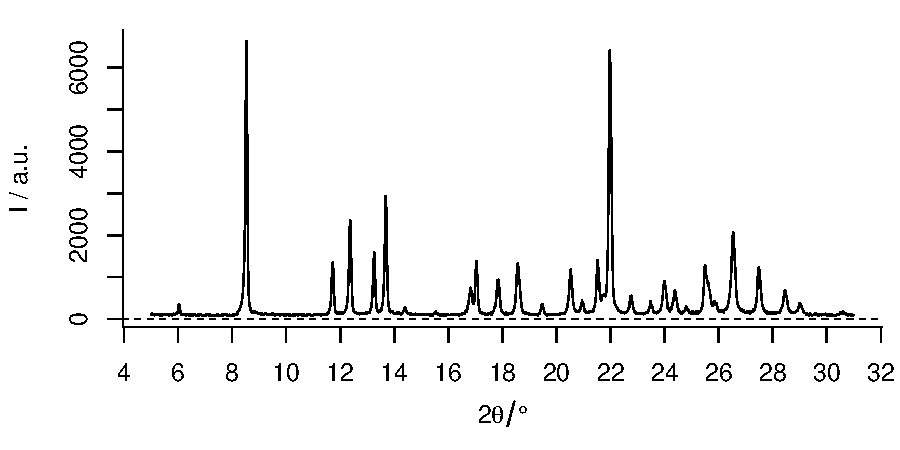
\includegraphics{fileio-fig--plot-triazine}

Witec also saves ASCII data with spectra in columns (Export $\rightarrow$ Table), see \ref{sec:read.txt.Witec}.

\subsection{JCAMP-DX}
\label{sec:jcamp-dx}
\index{ASCII!JCAMP-DX}
\index{JCAMP-DX!ASCII}
\index{jdx|see{JCAMP-DX}}
\index{JCAMP-DX!ASCII}
%
\label{sec:read.jdx}
\index{JCAMP-DX!Shimadzu} \index{Shimadzu!GC-MS}
\index{Shimadzu!JCAMP-DX} \index{JCAMP-DX!PerkinElmer} \index{PerkinElmer!JCAMP-DX}
\index{PerkinElmer!Infrared} \index{Infrared!PerkinElmer}
\index{JCAMP-DX!Infrared} \index{Infrared!JCAMP-DX}
%
Limited import of JCAMP-DX files v. 4.24 \cite{McDonald1988} is available in function
\Rfunction{read.jdx}.  These files can contain multiple spectra, supported data formats are tabular
\texttt{XY..XY} and \texttt{X++(Y..Y)}.
\begin{Schunk}
\begin{Sinput}
> read.jdx ("jcamp-dx/shimadzu.jdx", encoding = "latin1", keys.hdr2data=TRUE)
\end{Sinput}
\begin{Soutput}
hyperSpec object
   44 spectra
   12 data columns
   3401 data points / spectrum
wavelength:  [numeric] 59.7 59.9 ... 550.4 
data:  (44 rows x 12 columns)
   1. spc:  [matrix, array3401] NA NA ... NA + NA
   2. file:  [character] jcamp-dx/shimadzu.jdx jcamp-dx/shimadzu.jdx ... jcamp-dx/shimadzu.jdx 
   3. title:  [character] 1 2 ... 44 
   4. mw:  [numeric] 261 249 ... 382 
   5. molform:  [character] C11 H27 N O2 Si2 C9 H23 N O3 Si2  ... C25 H50 O2 
   6. casregistryno:  [character] 72 - 18 - 4 56 - 45 - 1 ... 2442 - 49 - 1 
   7. datatype:  [character] Mass Spectrum Mass Spectrum ... Mass Spectrum 
   8. sampledescription:  [character] ...\11-12-12\pAS+OS Lauf1.qgd"\n20000 Da/s, ET 30ms, m/z 60-550\nPeak-Apex-Spektrum, Hintergrund subtrahiert ...\11-12-12\pAS+OS Lauf1.qgd"\n20000 Da/s, ET 30ms, m/z 60-550\nPeak-Apex-Spektrum, Hintergrund subtrahiert ... ...\11-12-12\pAS+OS Lauf1.qgd"\n20000 Da/s, ET 30ms, m/z 60-550\nPeak-Apex-Spektrum, Hintergrund subtrahiert 
   9. casname:  [character] L-Valin N,O-TMS2      L-Serin O,O'-TMS2 (X) ... Methyltetracosanoat (LRI C24) 
   10. $retentionindex:  [numeric] 884 925 ... 2400 
   11. .format:  [character] (XY..XY) (XY..XY) ... (XY..XY) 
   12. filename: filename [character] jcamp-dx/shimadzu.jdx jcamp-dx/shimadzu.jdx ... jcamp-dx/shimadzu.jdx 
\end{Soutput}
\begin{Sinput}
> read.jdx ("jcamp-dx/virgilio.jdx")
\end{Sinput}
\begin{Soutput}
hyperSpec object
   1 spectra
   2 data columns
   1216 data points / spectrum
wavelength: tilde(nu)/cm^-1 [numeric] 3030 3028 ... 600 
data:  (1 rows x 2 columns)
   1. spc: A [matrix, array1216] -3.1244e-05 0.0000e+00 ... 0 
   2. filename: filename [character] jcamp-dx/virgilio.jdx 
\end{Soutput}
\end{Schunk}

The last file has a slight inconsistenty between its meta data and spectroscopic data,
causing a message.
However, the difference is minute compared to the intensities. If this is known in advance, an
appropriate tolerance can be chosen:
\begin{Schunk}
\begin{Sinput}
> read.jdx ("jcamp-dx/virgilio.jdx", ytol = 1e-9)
\end{Sinput}
\begin{Soutput}
hyperSpec object
   1 spectra
   2 data columns
   1216 data points / spectrum
wavelength: tilde(nu)/cm^-1 [numeric] 3030 3028 ... 600 
data:  (1 rows x 2 columns)
   1. spc: A [matrix, array1216] -3.1244e-05 0.0000e+00 ... 0 
   2. filename: filename [character] jcamp-dx/virgilio.jdx 
\end{Soutput}
\end{Schunk}

\warnbox{Note}{\Rfunction{read.jdx.Shimadzu} has been removed.}
\warnbox{Note}{An R package dedicated to importing JCAMP-DX is currently under development by Bryan Hanson
(\url{https://github.com/bryanhanson/readJDX}).
\phy will use that package once it is available on CRAN. Maintenance of \phy's \Rfunction{read.jdx} function
is limited from now on in favor of Bryan's pacakge.}

\subsection{Basic Atomic Spectra from NIST Tables}
\label{sec:aes-nist}
\index{ASCII!reference!atomic emission!NIST}
\index{atomic emission!NIST}
\index{NIST!atomic emission}
\index{reference!NIST!atomic emission}

The NIST (National Institute of Standards and Technology) has published a data base of basic atomic
emission spectra (see \url{http://physics.nist.gov/PhysRefData/Handbook/periodictable.htm})\cite{HandbookofBasicAtomicSpectroscopicData} with emission lines tabulated in
ASCII (HTML) files.

Here's an example how to extract the data of the Hg strong lines file:
\begin{Schunk}
\begin{Sinput}
> file <- readLines("NIST/mercurytable2.htm")
> #file <- readLines("http://physics.nist.gov/PhysRefData/Handbook/Tables/mercurytable2.htm")
> 
> file <- file [- (1 : grep ("Intensity.*Wavelength", file) - 1)]
> file <- file [1 : (grep ("</pre>", file) [1] - 1)]
> file <- gsub ("<[^>]*>", "", file)
> file <- file [! grepl ("^[[:space:]]+$", file)]
> colnames <- file [1]
> colnames <- gsub ("[[:space:]][[:space:]]+", "\t",  file [1])
> colnames <- strsplit (colnames, "\t")[[1]]
> if (! all (colnames == c ("Intensity", "Wavelength (&Aring;)", "Spectrum", "Ref. ")))
+   stop ("file format changed!")
> tablestart <- grep ("^[[:blank:]]*[[:alpha:]]+$", file) + 1
> tableend   <- c (tablestart [-1] - 2, length (file))
> tables <- list ()
> for (t in seq_along (tablestart)){
+   tmp <- file [tablestart [t] : tableend [t]]
+   tables [[t]] <- read.fwf (textConnection (tmp), c (5, 8, 12, 15, 9), stringsAsFactors = TRUE)
+   colnames (tables [[t]]) <- c("Intensity", "persistent", "Wavelength", "Spectrum", "Ref. ")
+   tables [[t]]$type <- gsub ("[[:space:]]", "", file [tablestart [t] - 1])
+ }
> tables <- do.call (rbind, tables)
> levels (tables$Spectrum) <- gsub (" ", "", levels (tables$Spectrum))
> Hg.AES <- list ()
> for (s in levels (tables$Spectrum))
+   Hg.AES [[s]] <- new ("hyperSpec", wavelength = tables$Wavelength [tables$Spectrum == s],
+                        spc = tables$Intensity [tables$Spectrum == s],
+                        data = data.frame (Spectrum = s),
+                        label = list (.wavelength = expression (lambda / ring (A)),
+                                       spc = "I"))
> plot (collapse (Hg.AES), lines.args = list (type = "h"), col = 1 : 2)
\end{Sinput}
\end{Schunk}
\subsection{Further ASCII Formats}
Further import filters are provided for manufacturer/software specific ASCII formats,
see table~\ref{sec:format} (p.~\pageref{sec:format}) and section~\ref{sec:manuf-spec-import}
(p.~\pageref{sec:manuf-spec-import}).

\subsection{ASCII Export}
ASCII export can be done in wide and long format using \Rfunction{write.txt.long} and
\Rfunction{write.txt.wide}. If you need a specific header or footer, use R's functions for writing
files: \Rfunction{write.table}, \Rfunction{write}, \Rfunction{cat} and so on offer fine-grained
control of writing ASCII files.

\section{Binary file formats}
\label{sec:binary-file-formats}

\subsection{Matlab Files}
\label{sec:readMat}
\index{Matlab}
Matlab files can be read and written using the package \Rpackage{R.matlab}\citep{R.matlab},
which is available at CRAN and can be installed by \Rcode{install.packages (\textquotedbl
R.matlab\textquotedbl)}.
\begin{Schunk}
  \begin{Sinput}
spc.mat <- readMat ("spectra.mat")
\end{Sinput}
\end{Schunk}

If the .mat file was saved with compression, the additional package \Rpackage{Rcompression} is
needed. It can be installed from omegahat:
\begin{Schunk}
  \begin{Sinput}
install.packages("Rcompression", repos = "http://www.omegahat.org/R")
\end{Sinput}
\end{Schunk}
See the documentation of \Rpackage{R.matlab} for more details and possibly needed further packages.

\Rfunction{readMat} imports the .mat file's contents as a list. The variables in the .mat file are
properly named elements of the list. The \chy object can be created using \Rfunction{new},
see~\ref{sec:new}~(p.~\pageref{sec:new}).

Again, you probably want to wrap the import of your matlab files into a function.

\subsubsection{Matlab Export}
\label{sec:writing-matlab-files}
\Rpackage{R.matlab}'s function \Rfunction{writeMat} can be used to write R objects into .mat files.
To save an \chy object \Robject{x} for use in Matlab, you most likely want to save:
\begin{itemize}
\item the wavelength axis as obtained by \Rcode{wl (x)},
\item the spectra matrix as obtained by \Rcode{x [[]]}, and
\item possibly also the extra data as obtained by \Rcode{x\$..}
\item as well as the axis labels \Rcode{labels (x)}.
\item Alternatively, \Rcode{x\$.} yields the extra data together with the spectra matrix.
\end{itemize}
However, it may be convenient to transform the saved data according to how it is needed in Matlab.
The functions \Rfunction{as.long.df} and \Rfunction{as.wide.df} may prove useful for reshaping the
data.
\subsubsection{Import of Matlab files written by Cytospec}
\label{sec:read.mat.Cytospec}
\index{Cytospec}\index{Cytospec!Matlab}\index{Matlab!Cytospec}

A custom import function for .mat files written by \href{www.cytospec.com}{Cytospec} is available:

Note that Cytospec files can contain multiple versions of the data, the so-called blocks. The block
to be read can be specified with the \Rfunarg{block} argument. \Rcode{TRUE} will read all blocks into
a list:

\begin{Schunk}
\begin{Sinput}
> read.mat.Cytospec ("mat.cytospec/cytospec.mat", blocks = TRUE)
\end{Sinput}
\begin{Soutput}
[[1]]
hyperSpec object
   55 spectra
   5 data columns
   981 data points / spectrum
wavelength:  [numeric] 499.12 501.77 ... 3100 
data:  (55 rows x 5 columns)
   1. x:  [integer] 4 5 ... 7 
   2. y:  [integer] 1 1 ... 11 
   3. block:  [integer] 1 1 ... 1 
   4. spc:  [matrix, array981] 2112.9 2114.3 ... 2323.3 
   5. filename: filename [character] mat.cytospec/cytospec.mat mat.cytospec/cytospec.mat ... mat.cytospec/cytospec.mat 

[[2]]
hyperSpec object
   55 spectra
   5 data columns
   981 data points / spectrum
wavelength:  [numeric] 499.12 501.77 ... 3100 
data:  (55 rows x 5 columns)
   1. x:  [integer] 4 5 ... 7 
   2. y:  [integer] 1 1 ... 11 
   3. block:  [integer] 2 2 ... 2 
   4. spc:  [matrix, array981] 58.472 59.024 ... 262.5 
   5. filename: filename [character] mat.cytospec/cytospec.mat mat.cytospec/cytospec.mat ... mat.cytospec/cytospec.mat 
\end{Soutput}
\end{Schunk}

otherwise, select a block:
\begin{Schunk}
\begin{Sinput}
> read.mat.Cytospec ("mat.cytospec/cytospec.mat", blocks = 1)
\end{Sinput}
\begin{Soutput}
hyperSpec object
   55 spectra
   5 data columns
   981 data points / spectrum
wavelength:  [numeric] 499.12 501.77 ... 3100 
data:  (55 rows x 5 columns)
   1. x:  [integer] 4 5 ... 7 
   2. y:  [integer] 1 1 ... 11 
   3. block:  [integer] 1 1 ... 1 
   4. spc:  [matrix, array981] 2112.9 2114.3 ... 2323.3 
   5. filename: filename [character] mat.cytospec/cytospec.mat mat.cytospec/cytospec.mat ... mat.cytospec/cytospec.mat 
\end{Soutput}
\end{Schunk}



\warnbox{\Rcode{read.cytomat} is now \textbf{defunct}.}{%
\Rcode{read.cytomat} has been renamed to  \Rcode{read.mat.Cytospec} to be more
consistent with the general naming scheme of the file import functions.

Please use \Rcode{read.mat.Cytospec} instead.
}

\subsection{ENVI Files}
\label{sec:read.ENVI}
\index{ENVI!Map} \index{ENVI!Infrared} \index{ENVI!Bruker} \index{ENVI!Varian} \index{Map!ENVI}
\index{Infrared!ENVI} \index{Bruker!ENVI} \index{Varian!ENVI} \index{FT-IR|see{Infrared}}
\index{Image|see{Map}} ENVI files are binary data accompanied by an ASCII header file. \phy's
function \Rfunction{read.ENVI} can be used to import them. Usually, the header file name is the same
as the binary data file name with the suffix replaced by {.}hdr. Otherwise, the header file name can
be given via parameter \textbf{\Rfunarg{headerfile}}.

As we experienced missing header files (Bruker's Opus software frequently produced header files
without any content), the data that would usually be read from the header file can also be handed to
\Rfunction{read.ENVI} as a list in parameter \textbf{\Rfunarg{header}}.  Arguments given in
\Rfunarg{header} replace corresponding entries of the header file. The help page gives details on
what elements the list should contain, see also the discussion of ENVI files written by Bruker's OPUS
software (section~\ref{sec:read.ENVI.Bruker}, p.~\pageref{sec:read.ENVI.Bruker}).

Here is how to use \Rfunction{read.ENVI}:
\begin{Schunk}
\begin{Sinput}
> spc <- read.ENVI ("ENVI/example2.img")
> spc
\end{Sinput}
\begin{Soutput}
hyperSpec object
   0 spectra
   3 data columns
   1738 data points / spectrum
wavelength:  [numeric] 649.90 651.83 ... 3999.7 
data:  (0 rows x 3 columns)
   1. x:  [integer]
   2. y:  [integer]
   3. spc:  [matrix, array1738]
\end{Soutput}
\end{Schunk}

Please see also the manufacturer specific notes in section~\ref{sec:manuf-spec-import},
p.~\pageref{sec:manuf-spec-import}.

\subsubsection{ENVI Export}
\label{sec:envi-export}
Use package \Rpackage{caTools} or \Rpackage{rgdal} with GDAL for writing ENVI files.

\subsection{spc Files}
\label{sec:read.spc}
\index{spc}
\index{spc!Raman}
\index{spc!Renishaw}
\index{spc!Kaiser}
\index{spc!TriVista}
\index{Raman!spc}
\index{Raman!Kaiser}
\index{Raman!HoloGram}
\index{Raman!LabRam}
\index{Raman!LabSpec}
\index{Raman!Horiba}
\index{Raman!Renishaw}
\index{Renishaw!spc}
\index{TriVista!spc}
\index{Horiba!spc}
\index{LabSpec!spc}
\index{LabRam!spc}
\index{Kaiser!spc}

Thermo Galactic's .spc file format can be imported by \Rfunction{read.spc}.

\warnbox[blue]{Official File Format Documentation}{The specification used to be available at Thermo Scientific. Anyone knowing where it moved
please contact me (\mailme) --- I'm looking for a reasonably official website (i.e. at Thermo)
rather than some random site with a copy.}
% TODO: find out via Massimiliano

A variety of sub-formats exists. \phy's import function \Rfunction{read.spc} does \emph{not} support
the old file format that was used before 1996. In addition, no test data with \emph{w planes} was
available --- thus the import of such files could not be tested. If you come across such files,
please contact the package maintainer (\mailme).

The header and subheader blocks of spc files store additional information of pre-defined types (see
the file format specification\cite{Galactic1997}). Further information can be stored in the so-called
log block at the end of the file, and should be in a key-value format (although even the official
example files do not always).  This information is often useful (Kaiser's Hologram software \eg
stores the stage position in the log block).

\Rfunction{read.spc} has four arguments that allow fine-grained control of storing such information
in the \chy object:
\begin{labeling}{\Rcode{keys.hdr2data}}
\item[\Rcode{keys.hdr2data}] parameters from the spc file and subfile headers that should become
  extra data columns
\item[\Rcode{keys.log2data}] parameters from the spc file log block that should become extra data
  columns
\item[\Rcode{keys.*2log}] parameters are deprecated because the logbook itself is depecated
\end{labeling}
The value of these arguments can either be logical (amounting to either use all or none of the
information in the file) or a character vector giving the names of the parameters that should be
used. Note that the header file field names are always lowercase.

Here's how to find out what extra information could be read from the header and log:

\begin{Schunk}
\begin{Sinput}
> read.spc ("spc.Kaisermap/ebroAVII.spc", keys.hdr2data = TRUE)
\end{Sinput}
\begin{Soutput}
hyperSpec object
   1 spectra
   34 data columns
   1340 data points / spectrum
wavelength: x/"a. u." [numeric] 1 2 ... 1340 
data:  (1 rows x 34 columns)
   1. z: x/"a. u." [numeric] 1 
   2. z.end: x/"a. u." [numeric] 1 
   3. ftflgs:  [matrix, array8] FALSE FALSE ... FALSE 
   4. fexper:  [factor] General 
   5. fexp:  [integer] -128 
   6. fnpts:  [integer] 1340 
   7. ffirst:  [numeric] 1 
   8. flast:  [numeric] 1340 
   9. fnsub:  [integer] 1 
   10. fxtype:  [character] x/"a. u." 
   11. fytype:  [character] Counts 
   12. fztype:  [character] x/"a. u." 
   13. fpost:  [integer] 0 
   14. fdate:  [POSIXct, POSIXt] 1253590860 
   15. fres:  [character]  
   16. fsource:  [character]  
   17. fspare:  [matrix, array8] 0 0 ... 0 
   18. fcmnt:  [character]  
   19. fcatxt:  [character]  
   20. flogoff:  [integer] 5904 
   21. fmods:  [integer] 0 
   22. fprocs:  [integer] 0 
   23. flevel:  [integer] 0 
   24. fsampin:  [integer] 0 
   25. ffactor:  [numeric] 0 
   26. fmethod:  [character]  
   27. fzinc:  [numeric] 0 
   28. fwplanes:  [integer] 0 
   29. fwinc:  [numeric] 0 
   30. fwtype:  [character] x/"a. u." 
   31. .last.read:  [numeric] 512 
   32. subfiledir:  [numeric] 0 
   33. spc: Counts [matrix, array1340] 2782.7 2229.8 ... 932.02 
   34. filename: filename [character] spc.Kaisermap/ebroAVII.spc 
\end{Soutput}
\begin{Sinput}
> read.spc ("spc.Kaisermap/ebroAVII.spc", keys.log2data = TRUE)
\end{Sinput}
\begin{Soutput}
hyperSpec object
   1 spectra
   55 data columns
   1340 data points / spectrum
wavelength: x/"a. u." [numeric] 1 2 ... 1340 
data:  (1 rows x 55 columns)
   1. z: x/"a. u." [numeric] 1 
   2. z.end: x/"a. u." [numeric] 1 
   3. Grams_File_Name:  [character] d:\beleites\ebro\Map 20090921 180944\ebroAVII.spc 
   4. HoloGRAMS_File_Name:  [character] Unknown 
   5. Acquisition_Date_Time:  [character] 22.09.2009 03:41:30 
   6. Lambda:  [character] Low 
   7. Accuracy_Mode:  [character] High Speed 
   8. Dark_subtracted:  [character] Yes 
   9. Dark_File_Name:  [character] ebroAVGC.drk 
   10. Auto_New_Dark_Curve:  [character] No 
   11. Background_subtracted:  [character] No 
   12. Background_File_Name:  [character] <None> 
   13. Intensity_Corrected:  [character] Yes 
   14. Intensity_Calibration_Available:  [character] Yes 
   15. Intensity_Correction_File:  [character] c:\hologram\calibration\intensity\20090609aa.icl 
   16. Intensity_Correction_Threshold:  [character] 0,00% 
   17. Intensity_Source_Correction:  [character] No 
   18. Intensity_Source_Correction_File:  [character] <None> 
   19. Comment:  [character] <None> 
   20. Cosmic_Ray_Filtering:  [character] Yes 
   21. Total_Cosmic_Count:  [character] 38 
   22. Exposure_Length:  [character] 10000 
   23. Accumulations:  [character] 1 
   24. Accumulation_Method:  [character] Averaged 
   25. Calibration_File:  [character] C:\HoloGRAM\calibration\Wavelength\20090716ab.wcl 
   26. Comment.1:  [character]  
   27. Temperature_Status:  [character] At temperature 
   28. Temperature:  [character] -85,50 
   29. HoloGRAMS_File_Version:  [character] 4.1 
   30. File_Type:  [character] Hol 
   31. Operator:  [character] unknown 
   32. Stage_X_Position:  [character] 360 
   33. Stage_Y_Position:  [character] 1100 
   34. Stage_Z_Position:  [character] -16 
   35. AutoFocusUsed:  [character] Nein 
   36. WLInterval:  [character] 0,12 
   37. CalInterval:  [character] 0,90 
   38. FFTFillFactor:  [character] None 
   39. FFTApT:  [character] None 
   40. SamplingMethod:  [character] Linear 
   41. Has_MultiPlex_Laser:  [character] No 
   42. External_Trigger:  [character] No 
   43. Laser_Wavelength:  [character] 785,21 
   44. Default_Laser_Wavelength:  [character] 785,21 
   45. Laser_Tracking:  [character] False 
   46. Laser_Block_Active:  [character] No 
   47. Pixel_Fill_minimum:  [character] 26 
   48. Pixel_Fill_maximum:  [character] 16762 
   49. Binning_Start:  [character] 24 
   50. Binning_End:  [character] 41 
   51. NumPoints:  [character] 1340 
   52. First:  [character] 1,000 
   53. last:  [character] 1340,000 
   54. spc: Counts [matrix, array1340] 2782.7 2229.8 ... 932.02 
   55. filename: filename [character] spc.Kaisermap/ebroAVII.spc 
\end{Soutput}
\end{Schunk}


.spc files may contain multiple spectra that do \emph{not} share a common wavelength axis. In this
case, \Rfunction{read.spc} returns a list of \chy objects with one spectrum
each. \Rfunction{collapse} may be used to combine this list into one \chy object:
\begin{Schunk}
\begin{Sinput}
> barbiturates <- read.spc ("spc/BARBITUATES.SPC")
> save (barbiturates, file = "barbiturates.rda")
> class (barbiturates)
\end{Sinput}
\begin{Soutput}
[1] "list"
\end{Soutput}
\begin{Sinput}
> length (barbiturates)
\end{Sinput}
\begin{Soutput}
[1] 286
\end{Soutput}
\begin{Sinput}
> barbiturates <- collapse (barbiturates, collapse.equal = FALSE)
> barbiturates
\end{Sinput}
\begin{Soutput}
hyperSpec object
   286 spectra
   4 data columns
   375 data points / spectrum
wavelength: frac(m, z)/frac(u, e) [numeric] 25.95 26.05 ... 244.05 
data:  (286 rows x 4 columns)
   1. z: t/min [numeric] 4.0272 4.0341 ... 5.9978 
   2. z.end: t/min [numeric] 4.0272 4.0341 ... 5.9978 
   3. spc: I/"a. u." [matrix, array375] NA NA ... NA + NA
   4. filename: filename [character] spc/BARBITUATES.SPC spc/BARBITUATES.SPC ... spc/BARBITUATES.SPC 
\end{Soutput}
\begin{Sinput}
> barbiturates [[1:10, , 25 ~ 30]]
\end{Sinput}
\begin{Soutput}
      25.95 26.05 26.15 26.95 27.05 27.15 28.05 28.15 29.05 29.15 29.95
 [1,]    NA    NA    NA    NA   562    NA    NA 11511  6146    NA    NA
 [2,]    NA    NA    NA    NA    NA   618 10151    NA  5040    NA    NA
 [3,]    NA    NA    NA    NA   638    NA    NA 10722  5253    NA    NA
 [4,]    NA    NA    NA    NA    NA    NA 10548    NA  5865    NA    NA
 [5,]    NA    NA    NA    NA    NA    NA    NA 10519  4664    NA    NA
 [6,]    NA    NA    NA   796    NA    NA 10519    NA  5110    NA    NA
 [7,]    NA    NA    NA    NA    NA    NA 10096    NA  4769    NA   907
 [8,]    NA    NA    NA    NA    NA    NA    NA 10929  5400    NA    NA
 [9,]    NA    NA    NA    NA    NA    NA 10235    NA  4930    NA    NA
[10,]    NA    NA    NA    NA    NA    NA    NA 10663  4690    NA   799
\end{Soutput}
\end{Schunk}

\paragraph{Deriving manufacturer specific import filters.}
Please note that future changes inside the read.spc function are likely to occur.  However, if you
just post-process the \chy object returned by \Rfunction{read.spc}, you should be fine.

\section{Manufacturer-Specific Discussion of File Import}
\subsection{Manufacturer Specific Import Functions}
\label{sec:manuf-spec-import}
Many spectrometer manufacturers provide a function to export their spectra into ASCII files. The
functions discussed above are written in a very general way, and are highly customizable.  I
recommend wrapping these calls with the appropriate settings for your spectra format in an import
function. Please consider contributing such import filters to \Rpackage{hyperSpec}: send me the
documented code (for details see the box at the beginning of this document).  If you are able to
import data of any format not mentioned in this document (even without the need of new converters),
please let me know (details again in the box at the beginning of this document).

\subsection{Bruker FT-IR Imaging}
\label{sec:read.ENVI.Bruker}
\index{ENVI!Map}
\index{ENVI!Infrared}
\index{ENVI!Bruker}
\index{Map!ENVI}
\index{Infrared!ENVI}
\index{Bruker!ENVI}

We use \Rfunction{read.ENVI} to import IR-Images collected with a Bruker Hyperion spectrometer with
OPUS software. As mentioned above, the header files are frequently empty. We found the necessary
information to be:
\begin{Schunk}
\begin{Sinput}
> header <- list (samples = 64 * no.images.in.row,
+                 lines = 64 * no.images.in.column,
+                 bands = no.data.points.per.spectrum,
+                 `data type` = 4,
+                 interleave = "bip")
\end{Sinput}
\end{Schunk}
No spatial information is given in the ENVI header (if written). The lateral coordinates can be setup
by specifying origin and pixel size for $x$ and $y$ directions. For details please see the help page.

The proprietary file format of the Opus software is not yet supported.

\subsection{Nicolet FT-IR Imaging}
\label{sec:read.ENVI.Nicolet}
\index{ENVI!Map}
\index{ENVI!Infrared}
\index{ENVI!Nicolet}
\index{Map!ENVI}
\index{Infrared!ENVI}
\index{Nicolet!ENVI}

Also Nicolet saves imaging data in ENVI files. These files use some non-standard keywords in the
header file that should allow to reconstruct the lateral coordinates as well as the wavelength axes
and units for wavelength and intensity axis. \phy has a specialized function
\Rfunction{read.ENVI.Nicolet} that uses these header entries.

It seems that the position of the first spectrum is recorded in \mum{}, while the pixel size is in
mm. Thus a flag \Rfunarg{nicolet.correction} is provided that divides the pixel size by 1000.
Alternatively, the correct offset and pixel size values may be given as function arguments.

\begin{Schunk}
\begin{Sinput}
> spc <- read.ENVI.Nicolet ("ENVI/example2.img", nicolet.correction = TRUE)
> spc ## dummy sample with all intensities zero
\end{Sinput}
\begin{Soutput}
hyperSpec object
   0 spectra
   3 data columns
   1738 data points / spectrum
wavelength:  [numeric] 649.90 651.83 ... 3999.7 
data:  (0 rows x 3 columns)
   1. x:  [numeric]
   2. y:  [numeric]
   3. spc:  [matrix, array1738]
\end{Soutput}
\end{Schunk}

\subsection{Varian/Agilent FT-IR Imaging}
\label{sec:varianagilent-ft-ir}
\index{ENVI!Map}
\index{ENVI!Infrared}
\index{ENVI!Agilent}
\index{Map!ENVI}
\index{Infrared!ENVI}
\index{Agilent!ENVI}
\index{Varian|see{Agilent}}

Agilent (Varian) uses a variant of ENVI (with binary header).

\subsection{Kaiser Optical Systems Raman}
\label{sec:Kaiser}
\index{spc!Raman}
\index{spc!Kaiser}
\index{hol!Kaiser}
\index{Raman!spc}
\index{Raman!Kaiser}
\index{Raman!hol}
\index{Kaiser!hol}
\index{Kaiser!spc}

Spectra obtained using Kaiser's Hologram software can be saved either in their own .hol format and
imported into Matlab (from where the data may be written to a .mat file readable by
\Rpackage{R.matlab}'s \Rfunction{readMat}. Hologram can also write ASCII files and .spc files. We
found working with .spc files the best option.

The spectra are usually interpolated by Hologram to an evenly spaced wavelength (or
$\Delta\tilde\nu$) axis unless the spectra are saved in a by-pixel manner. In this case, the full
spectra consist of two files with consecutive file names: one for the low and one for the high
wavenumber region. See the example for .spc import.

\subsubsection{Kaiser Optical Systems ASCII Files}
\label{sec:KaiserASCII}
\index{ASCII!long!Raman}
\index{ASCII!long!Kaiser}
\index{Raman!Kaiser}
\index{Raman!ASCII long}
\index{Kaiser!ASCII long}

The ASCII files are long format that can be imported by \Rfunction{read.txt.long} (see
section~\ref{sec:read.txt.long}, p.~\pageref{sec:read.txt.long}).

We experienced two different problems with these files:
\begin{compactenum}
\item If the instrument computer's locale is set so that also the decimal separator is a comma,
  commas are used both as decimal and as column separator.
\item Values with a decimal fraction of $0$ are written with decimal separator but no further digits
  (\eg \texttt{2,}). This may be a problem for certain conversion functions (\Rfunction{read.table}
  works fine, though).
\end{compactenum}

Thus care must be taken:
\begin{Schunk}
\begin{Sinput}
> ## 1. import as character
> tmp <- scan ("txt.Kaiser/test-lo-4.txt", what = rep ("character",4), sep = ",")
> tmp <- matrix (tmp, nrow = 4)
> ## 2. concatenate every two columns by a dot
> wl <- apply (tmp [1:2, ], 2, paste, collapse = '.')
> spc <- apply (tmp [3:4, ], 2, paste, collapse = '.')
> ## 3. convert to numeric and create hyperSpec object
> spc <- new ("hyperSpec", spc = as.numeric (spc), wavelength = as.numeric (wl))
\end{Sinput}
\end{Schunk}

\subsubsection{Kaiser Optical Systems Raman Maps}
\label{sec:read.spc.KaiserMap}
\index{Map}
\index{Map!Raman}
\index{Map!Kaiser}
\index{Raman!Map}
\index{Raman!Kaiser}
\index{Raman!spc}
\index{Kaiser!Map}
\index{Kaiser!spc}

\phy provides the function \Rfunction{read.spc.KaiserMap} to easily import spatial collections of
.spc files written by Kaiser's Hologram software. The filenames of all .spc files to be read into one
\chy object can be provided either as a character vector or as a wildcard expression (\eg
\textquotedbl path/to/files/*.spc\textquotedbl ).

The data for the following example was saved with wavelength axis being camera pixels rather than
Raman shift. Thus two files for each spectrum were saved by Hologram. Thus, a file name pattern is
difficult to give and a vector of file names is used instead:
\begin{Schunk}
\begin{Sinput}
> files <- Sys.glob ("spc.Kaisermap/*.spc")
> spc.low <- read.spc.KaiserMap (files [seq (1, length (files), by = 2)])
> spc.high <- read.spc.KaiserMap (files [seq (2, length (files), by = 2)])
> wl (spc.high) <- wl (spc.high) + 1340
> spc
\end{Sinput}
\begin{Soutput}
hyperSpec object
   1 spectra
   1 data columns
   2110 data points / spectrum
wavelength:  [numeric] 121.5 122.4 ... 2019.6 
data:  (1 rows x 1 columns)
   1. spc:  [matrix, array2110] 1202.51 770.35 ... 141.01 
\end{Soutput}
\end{Schunk}

\subsection{Renishaw Raman}
\label{sec:read.txt.renishaw}
\index{Raman!Renishaw!spc}
\index{Renishaw!Raman}
\index{Renishaw!spc}
\index{spc!Renishaw}
\index{spc!Raman}

Renishaw's Wire software comes with an file format converter. This program can produce a long ASCII
format, .spc, or .jdx files.

We experienced that the conversion to .spc is \emph{not} fully reliable: maps were saved as depth
profile, loosing all spatial information. In addition, an evenly spaced wavelength axis was produced,
although this was de-selected in the converter. We therefore recommend using the ASCII format.
Otherwise the import using \Rfunction{read.spc} worked.

\subsubsection{Renishaw ASCII data}
\label{sec:read.txt.Renishaw}
\index{ASCII!long!Raman}
\index{ASCII!long!Renishaw}
\index{ASCII!compressed}
\index{ASCII!zip}
\index{Raman!ASCII long}
\index{Raman!Renishaw!ASCII}
\index{Renishaw!Raman}
\index{Renishaw!ASCII long}
%
An optimized import function for the ASCII files is available: \Rfunction{read.txt.Renishaw}. The
file may be compressed via gzip, bzip2, xz or lzma. zip compressed files are read via
\Rfunction{read.zip.Renishaw}.  The ASCII files can easily become very large, particularly with
linefocus- or streamline imaging.  \Rfunction{read.txt.Renishaw} provides two mechanisms to avoid
running out of memory during data import. The file may be imported in chunks of a given number of
lines (see the last example). \Rfunction{read.txt.Renishaw} can calculate the correct number of
wavelengths (\ie data points per spectrum) if the system command \texttt{wc} is available on your
computer.

In addition, the processing of the long ASCII format into the spectra matrix is done by reshaping the
vector of intensities into a matrix. This process does not allow any missing values in the data.
\emph{Therefore it is not possible to import multi-spectra files with individually ``zapped'' spectra
  using \Rfunction{read.txt.Renishaw}.}

The second argument to  \Rfunction{read.txt.Renishaw} decides what type of experiment is imported.
Supported types are:
\begin{labeling}{\Rcode{\textquotedbl depth\textquotedbl}, \Rcode{\textquotedbl zspc\textquotedbl}}
\item[\Rcode{\textquotedbl xyspc\textquotedbl}] maps, images, multiple spectra with $x$ and $y$
coordinates (default)
\item[\Rcode{\textquotedbl spc\textquotedbl}] single spectrum
\item[\Rcode{\textquotedbl depth\textquotedbl}, \Rcode{\textquotedbl zspc\textquotedbl}] depth series
\item[\Rcode{\textquotedbl ts\textquotedbl}] time series
\end{labeling}

Instead of a file name, \Rfunction{read.txt.Renishaw} accepts also a connection.

\begin{Schunk}
\begin{Sinput}
> paracetamol <- read.txt.Renishaw ("txt.Renishaw/paracetamol.txt", "spc")
> paracetamol
\end{Sinput}
\begin{Soutput}
hyperSpec object
   1 spectra
   2 data columns
   4064 data points / spectrum
wavelength: Delta * tilde(nu)/cm^-1 [numeric] 96.787 98.143 ... 3200.1 
data:  (1 rows x 2 columns)
   1. spc: I / a.u. [matrix, array4064] 2056.5 2224.8 ... 299.23 
   2. filename: filename [character] txt.Renishaw/paracetamol.txt 
\end{Soutput}
\begin{Sinput}
> save (paracetamol, file = "paracetamol.rda")
> read.txt.Renishaw ("txt.Renishaw/laser.txt.gz", "ts")
\end{Sinput}
\begin{Soutput}
hyperSpec object
   84 spectra
   3 data columns
   140 data points / spectrum
wavelength: Delta * tilde(nu)/cm^-1 [numeric] -199.08 -196.90 ... 99.934 
data:  (84 rows x 3 columns)
   1. t: t / s [numeric] 0 2 ... 5722 
   2. spc: I / a.u. [matrix, array140] 29.801 32.093 ... 81.3 
   3. filename: filename [character] txt.Renishaw/laser.txt.gz txt.Renishaw/laser.txt.gz ... txt.Renishaw/laser.txt.gz 
\end{Soutput}
\end{Schunk}

Very large files can  be read in chunks to save  memory:
\begin{Schunk}
\begin{Sinput}
> read.txt.Renishaw ("txt.Renishaw/chondro.txt", nlines = 1e5, nspc = 875)
\end{Sinput}
\begin{Soutput}
............
hyperSpec object
   875 spectra
   4 data columns
   1272 data points / spectrum
wavelength: Delta * tilde(nu)/cm^-1 [numeric] 601.62 602.66 ... 1802.2 
data:  (875 rows x 4 columns)
   1. y: y/(mu * m) [numeric] -4.77 -4.77 ... 19.23 
   2. x: x/(mu * m) [numeric] -11.55 -10.55 ... 22.45 
   3. spc: I / a.u. [matrix, array1272] 501.72 518.53 ... 151.92 + NA
   4. filename: filename [character] txt.Renishaw/chondro.txt txt.Renishaw/chondro.txt ... txt.Renishaw/chondro.txt 
\end{Soutput}
\end{Schunk}

R accepts a variety of compressed file formats for ASCII files:
\begin{Schunk}
\begin{Sinput}
> read.txt.Renishaw ("txt.Renishaw/chondro.gz")
> read.txt.Renishaw ("txt.Renishaw/chondro.xz")
> read.txt.Renishaw ("txt.Renishaw/chondro.lzma")
> read.txt.Renishaw ("txt.Renishaw/chondro.gz")
> read.txt.Renishaw ("txt.Renishaw/chondro.bz2")
> read.zip.Renishaw ("txt.Renishaw/chondro.zip")
\end{Sinput}
\end{Schunk}

\subsection{Horiba / Jobin Yvon (e.g. LabRAM) }
\label{sec:read.txt.Horiba}
\index{Horiba Jobin Yvon!ASCII!wide}
\index{ASCII!wide!Horiba Jobin Yvon}
\index{Raman!Horiba Jobin Yvon!ASCII wide}
\index{Horiba!ASCII!wide}
\index{ASCII!wide!Horiba}
\index{Raman!Horiba!ASCII wide}
\index{LabRAM|see{Horiba}}
\index{ASCII!wide!LabRAM|see{Horiba}}
\index{Raman!LabRAM|see{Horiba}}

Horiba's Labspec software (e.\,g. LabRAM spectrometers) saves spectra in a wide ASCII format which is
read by \Rfunction{read.txt.Horiba}, e.\,g.:
\begin{Schunk}
\begin{Sinput}
> spc <- read.txt.Horiba ("txt.HoribaJobinYvon/ts.txt",
+                       cols = list (t = "t / s", spc = "I / a.u.",
+                         .wavelength = expression (Delta * tilde (nu) / cm^-1))
+                       )
> spc
\end{Sinput}
\begin{Soutput}
hyperSpec object
   100 spectra
   3 data columns
   1024 data points / spectrum
wavelength: Delta * tilde(nu)/cm^-1 [numeric] 2135.2 2133.3 ... -122.41 
data:  (100 rows x 3 columns)
   1. t: t / s [numeric] 0.000 5.834 ... 566.77 
   2. spc: I / a.u. [matrix, array1024] 6244 6278 ... 117 
   3. filename: filename [character] txt.HoribaJobinYvon/ts.txt txt.HoribaJobinYvon/ts.txt ... txt.HoribaJobinYvon/ts.txt 
\end{Soutput}
\end{Schunk}

Note that Labspec .txt files can contains lots of spectra with zero intensity: Labspec saves a
complete rectangular grid even if only part of a map was measured. These spectra are by removed
by default if option \Rcode{file.remove.emptyspc} is \Rcode{TRUE} (the default).

For convenience, functions to further wrappers to import maps (\Rfunction{read.txt.Horiba.xy}) and
time series (\Rfunction{read.txt.Horiba.t}) are provided.

\subsection{Andor Solis}
\label{sec:read.asc.Andor}
\index{Andor Solis!ASCII}
\index{ASCII!Andor Solis}
\index{Raman!Andor Solis!ASCII}

Andor Solis exports ASCII files that can be read with \Rfunction{read.asc.Andor}:
\begin{Schunk}
\begin{Sinput}
> read.asc.Andor("asc.Andor/ASCII-Andor-Solis.asc")
\end{Sinput}
\begin{Soutput}
hyperSpec object
   5 spectra
   2 data columns
   63 data points / spectrum
wavelength:  [numeric] 161.41 165.73 ... 423.65 
data:  (5 rows x 2 columns)
   1. spc:  [matrix, array63] 3404 3402 ... 3415 
   2. filename: filename [character] asc.Andor/ASCII-Andor-Solis.asc asc.Andor/ASCII-Andor-Solis.asc asc.Andor/ASCII-Andor-Solis.asc asc.Andor/ASCII-Andor-Solis.asc asc.Andor/ASCII-Andor-Solis.asc 
\end{Soutput}
\end{Schunk}

\subsection{Witec}
\label{sec:read.txt.Witec}
\index{Witec!ASCII}
\index{ASCII!Witec}
\index{Graph ASCII!Witec}
\index{Witec!Graph ASCII}
\index{Raman!Witec!ASCII}
\index{Raman!Witec!Save ASCII X, Save ASCII Y}
\index{Raman!Witec!Export Table}
\index{Raman!Witec!spc}
\index{Raman!Witec!Graph ASCII}
\index{spc!Witec}

The Witec project software supports exporting spectra as Thermo Galactic \texttt{.spc} files.
\begin{Schunk}
\begin{Sinput}
> read.spc ("spc.Witec/Witec-timeseries.spc")
> read.spc ("spc.Witec/Witec-Map.spc")
\end{Sinput}
\end{Schunk}
\texttt{.spc} is in general the recommended format for \phy import. For imaging data no spatial information for the set of spectra is provided (in version 2.10 this export option is not supported).

Imaging data (but also single spectra and time series) can be exported as ASCII X and Y files (Save ASCII X and Save ASCII Y, not supported in version 4). These can be read by \Rfunction{read.dat.Witec}:
\begin{Schunk}
\begin{Sinput}
> read.dat.Witec ("txt.Witec/Witec-timeseries-x.dat")
> read.dat.Witec (filex = "txt.Witec/Witec-Map-x.dat",
+                 points.per.line = 5, lines.per.image = 5, type = "map")
\end{Sinput}
\end{Schunk}
Note that the Y data files also contain a wavelength information, but (at least Witec Project 2.10) this information is always wavelength in nm, not Raman shift in wavenumbers: this is provided by the X data file only.

Another option is Witec's txt table ASCII export (Export $\rightarrow$ Table), which produces ASCII files with each row corresponding to one wavelength. The first column contains the wavelength axis, all further columns contain one spectrum each column. Such files can be read with \Rfunction{read.txt.Witec}:
\begin{Schunk}
\begin{Sinput}
> read.txt.Witec ("txt.Witec/Witec-timeseries_no.txt")
\end{Sinput}
\end{Schunk}
\Rfunction{read.txt.Witec} determines the number of wavelengths automaticallly.

Note that there are several Export Filter Options. Here you can determine, which units should be used for the export (see XUnits tab). In addition, it is possible to export two additional header lines containing information about spectra labels and units. Therefore parameters \Rfunarg{hdr.label} and \Rfunarg{hdr.units} have to be set properly. Otherwise, either an error will be displayed like
\begin{Schunk}
\begin{Soutput}
Error in scan(file, what, nmax, sep, dec, quote, skip, nlines, na.strings,  :
  scan() expected 'a real', got 'rel.'
\end{Soutput}
\end{Schunk}
or the one or two wavelengths will be skipped.

Depending on the used export options the header files should look like:
\begin{Schunk}
\begin{Soutput}
with exported labels and units headerlines: 
X-Axis                         Time Series_000_Spec.Data 1(0) Time Series_000_Spec.Data 1(1) 
rel. 1/cm                      CCD cts                        CCD cts                        
 8.77367E+01                    9.95000E+02                    9.94000E+02                   
 9.10310E+01                    9.96000E+02                    9.94000E+02                   

with exported labels headerline: 
X-Axis                         Time Series_000_Spec.Data 1(0) Time Series_000_Spec.Data 1(1) 
 8.77367E+01                    9.95000E+02                    9.94000E+02                   
 9.10310E+01                    9.96000E+02                    9.94000E+02                   
 9.43239E+01                    9.92000E+02                    9.92000E+02                   

with exported units headerline: 
rel. 1/cm    CCD cts      CCD cts      
 8.77367E+01  9.95000E+02  9.94000E+02 
 9.10310E+01  9.96000E+02  9.94000E+02 
 9.43239E+01  9.92000E+02  9.92000E+02 

without headerline: 
 87.737 995.000 994.000 
 91.031 996.000 994.000 
 94.324 992.000 992.000 
 97.615 989.000 989.000 
\end{Soutput}
\end{Schunk}
For imaging data set parameter \Rfunarg{type} to "map". If the label header is exported, the spatial information can be extracted from this line. Otherwise, at least one, \Rfunarg{points.per.line} or \Rfunarg{lines.per.image}, has to be given manually, if not, a warning will be shown.

For line scans and z-stacks use \Rfunarg{type = "single"} because the provided information are looking the same like for timeseries, so no further information can be extracted from the header files.

Since version 4 WITec Project offers the Graph ASCII export (Export $\rightarrow$ Graph ASCII) which produces three ASCII files, named Header containing additional information, X-Axis containing the wavelength values and Y-Axis containing the spectra one spectrum in each column. Data exported in this way can be read with \Rfunction{read.txt.Witec.Graph}:
\begin{Schunk}
\begin{Sinput}
> read.txt.Witec.Graph ("txt.Witec/Witec-timeseries (Header).txt")
> read.txt.Witec.Graph ("txt.Witec/Witec-Map (Header).txt", type = "map")
> read.txt.Witec.Graph ("txt.Witec/nofilename (Header).txt", encoding = "latin1")
\end{Sinput}
\end{Schunk}
This function reads the spectra files automatically, if they are named properly and extracts additional information of the header file. As for the other Witec functions it is possible to read image data by by selecting \Rfunarg{type = "map"}. Line scans and z-stacks should be read as single spectra.

\section{Writing your own Import Function}
\label{sec:writing-Import}
This section gives examples how to write import functions. The first example implements an import
filter for an ASCII file format basically from scratch. The second example shows how to implement
more details for an already existing import filter.

\subsection{A new ASCII Import Function: read.txt.PerkinElmer}
\label{sec:read.txt.PerkinElmer}
\index{ASCII!long!Fluorescence}
\index{ASCII!long!PerkinElmer}
\index{Fluorescence!ASCII long}
\index{Fluorescence!PerkinElmer!ASCII}
\index{PerkinElmer!Fluorescence}
\index{PerkinElmer!ASCII long}
The raw spectra of the \Robject{flu} data set (see also the respective vignette) are in PerkinElmer's ASCII file format, one spectrum per file.

We need a function that automatically reads all files specified by a pattern, such as \texttt{*.txt}.
In order to gain speed, the spectra matrix should be preallocated after the first file is read.

A short examination of the files (\texttt{flu*.txt} in directory \texttt{txt.PerkinElmer}) reveals
that the actual spectrum starts at line 55, after a line containing \texttt{\#DATA}.
For now, no other information of the files is to be extracted. It is thus easier to skip the first 54
lines than searching for the line after \texttt{\#DATA}.

A fully featured import function should support:
\begin{itemize}
\item Reading multiple files by giving a pattern
\item hand further arguments to \Rfunction{scan}. This comes handy in case the function is used later
to import other data types.
\item Also skipping 54 lines would be a weird default, so we rather require it to be given
explicitly.
\item The same applies for the axis labels: they should default to reasonable settings for
fluorescence spectra, but it should be possible to change them if needed.
\item The usual log entry arguments should be supplied.
\item A sanity check should be implemented: stop with an error if a file does not have the same
wavelength axis as the others.
\item If no file can be found, an empty \chy object is a reasonable result: There is no need
to stop with an error, but it is polite to issue an additional warning.
\item Finally, \phy does some optional common post-processing for all imported files such as attaching the filename (or connection description) to the \chy object (column \Rcode{filename}) and deleting empty spectra. These options can be globally switched on or off by options.
\end{itemize}

\VerbatimInput[frame=single, label={read.txt.PerkinElmer.R},
formatcom=\footnotesize]{read.txt.PerkinElmer.R}

Note how the labels are set. The label with the special name \Rcode{.wavelength} corresponds to the
wavelength axis, all data columns should have a label with the same name. The spectra are always in a
data column called \Rcode{spc}.

Thus,
\begin{Schunk}
\begin{Sinput}
> source ("read.txt.PerkinElmer.R")
> read.txt.PerkinElmer (Sys.glob("txt.PerkinElmer/flu?.txt"), skip = 54)
\end{Sinput}
\begin{Soutput}
hyperSpec object
   6 spectra
   2 data columns
   181 data points / spectrum
wavelength: lambda/nm [numeric] 405.0 405.5 ... 495 
data:  (6 rows x 2 columns)
   1. spc: I[fl]/"a.u." [matrix, array181] 27.150 66.801 ... 294.65 
   2. filename: filename [character] txt.PerkinElmer/flu1.txt txt.PerkinElmer/flu2.txt ... txt.PerkinElmer/flu6.txt 
\end{Soutput}
\end{Schunk}
imports the spectra.

This function is not exported by \phy: while it is already useful for importing files, it is not yet
general enough to work immediately with new data, \eg the the file header is completely ignored. Thus
information like the excitation wavelength is lost.

\subsection{Deriving a More Specific Function: read.ENVI.Nicolet}
\index{Infrared!ENVI}
\index{Infrared!Map}
\index{Infrared!Nicolet}
\index{ENVI!Infrared!Nicolet}
\index{ENVI!Map}
\index{ENVI!Nicolet}
\index{Nicolet!ENVI}
\index{Nicolet!Map}
\index{Nicolet!Infrared}
The function \Rfunction{read.ENVI.Nicolet} is a good example for a more specific import filter
derived from a general filter for the respective file type.
Nicolet FT-IR Imaging software saves some non-standard keywords in the header file of the ENVI data.
These information can be used to reconstruct the $x$ and $y$ axes of the images. The units of the
spectra are saved as well.

\Rfunction{read.ENVI.Nicolet} thus first adjusts the parameters for \Rfunction{read.ENVI}. Then
\Rfunction{read.ENVI} does the main work of importing the file. The resulting \chy object is
post-processed according to the special header entries.

For using the function, see section~\ref{sec:read.ENVI.Nicolet}~(p.~\pageref{sec:read.ENVI.Nicolet}).
\VerbatimInput[frame=single, label={read.ENVI.Nicolet.R},
formatcom=\footnotesize]{read.ENVI.Nicolet.R}

\subsection{Deriving import filters for spc files}
Please note that future changes inside the read.spc function are likely to occur.
However, if you just post-process the \chy object returned by \Rfunction{read.spc}, you should be fine.

\bibliographystyle{unsrtnat}
\bibliography{fileio-pkg,fileio}

\clearpage
\appendix
\section{File Import  Functions by Format}
\label{sec:format}
\renewcommand{\arraystretch}{1.5}
\begin{footnotesize}
  \begin{tabular}{@{} l l l l >{\raggedright}p{3.4cm}}
  \textbf{Format} &
  \textbf{Manufacturer} &
  \textbf{Function} &
  \textbf{section}  &
  \textbf{Notes}\tabularnewline
  \multicolumn{4}{@{}l}{\emph{\textbf{ASCII file formats}}}\tabularnewline
Andor Solis ASCII & Andor (Raman) & \Rfunction{read.asc.Andor} & \ref{sec:read.asc.Andor}, p. \pageref{sec:read.asc.Andor} & \tabularnewline
ASCII long &  & \Rfunction{read.txt.long} & \ref{sec:read.txt.long}, p. \pageref{sec:read.txt.long} & \tabularnewline
ASCII long & Renishaw (Raman) & \Rfunction{read.txt.Renishaw} & \ref{sec:read.txt.Renishaw}, p. \pageref{sec:read.txt.Renishaw} & \tabularnewline
ASCII long & Kaiser (Raman) & \Rfunction{read.txt.long} & \ref{sec:KaiserASCII}, p. \pageref{sec:KaiserASCII} & \emph{Not} recommended, see discussion\tabularnewline
ASCII long & Perkin Elmer (Fluorescence) & \Rfunction{read.txt.PerkinElmer} & \ref{sec:read.txt.PerkinElmer}, p. \pageref{sec:read.txt.PerkinElmer} & Reads multiple files, needs to be sourced.\tabularnewline
ASCII wide &  & \Rfunction{read.txt.wide} & \ref{sec:read.txt.wide}, p. \pageref{sec:read.txt.wide} & \tabularnewline
ASCII wide & Horiba Jobin Yvon (Raman) & \Rfunction{read.txt.Horiba} & \ref{sec:read.txt.Horiba}, p. \pageref{sec:read.txt.Horiba} & e.\,g. LabRAM spectrometers\tabularnewline
ASCII wide & Horiba Jobin Yvon (Raman) & \Rfunction{read.txt.Horiba.xy} & \ref{sec:read.txt.Horiba}, p. \pageref{sec:read.txt.Horiba} & e.\,g. LabRAM spectrometer maps\tabularnewline
ASCII wide & Horiba Jobin Yvon (Raman) & \Rfunction{read.txt.Horiba.t} & \ref{sec:read.txt.Horiba}, p. \pageref{sec:read.txt.Horiba} & e.\,g. LabRAM spectrometer time series\tabularnewline
ASCII wide transposed & Witec (Raman) & \Rfunction{read.txt.Witec} & \ref{sec:read.txt.Witec}, p. \pageref{sec:read.txt.Witec} & Export Table\tabularnewline
JCAMP-DX &  & \Rfunction{read.jdx} & \ref{sec:jcamp-dx}, p. \pageref{sec:jcamp-dx} & \tabularnewline
JCAMP-DX & Renishaw (Raman) & \Rfunction{read.jdx} & \ref{sec:jcamp-dx}, p. \pageref{sec:jcamp-dx} & \tabularnewline
JCAMP-DX & Shimadzu (GCxGC-MS) & \Rfunction{read.txt.Shimadzu} & \ref{sec:}, p. \pageref{sec:} & \tabularnewline
JCAMP-DX & PerkinElmer (Infrared) & \Rfunction{read.jdx} & \ref{sec:jcamp-dx}, p. \pageref{sec:jcamp-dx} & import for subset of the JCAMP-DX standard\tabularnewline
other & Shimadzu (GC,GC-MS) & \Rfunction{read.jdx} & \ref{sec:jcamp-dx}, p. \pageref{sec:jcamp-dx} & import for  subset of the JCAMP-DX standard\tabularnewline
Witec ASCII & Witec (Raman) & \Rfunction{read.dat.Witec} & \ref{sec:read.txt.Witec}, p. \pageref{sec:read.txt.Witec} & Save ASCII X, Save ASCII Y\tabularnewline
Witec Graph ASCII & Witec (Raman) & \Rfunction{read.txt.Witec.Graph} & \ref{sec:read.txt.Witec}, p. \pageref{sec:read.txt.Witec} & Export Table in 3 separate files (Header, X-Axis, Y-Axis)\tabularnewline
zipped ASCII long & Renishaw (Raman) & \Rfunction{read.zip.Renishaw} & \ref{sec:read.txt.Renishaw}, p. \pageref{sec:read.txt.Renishaw} & \tabularnewline\multicolumn{4}{@{}l}{\emph{\textbf{binary file formats}}}\tabularnewline
array &  & \Rfunction{-} & \ref{sec:new}, p. \pageref{sec:new} & \tabularnewline
ENVI &  & \Rfunction{read.ENVI} & \ref{sec:read.ENVI}, p. \pageref{sec:read.ENVI} & \tabularnewline
ENVI & Bruker (Infrared Imaging) & \Rfunction{read.ENVI} & \ref{sec:read.ENVI.Bruker}, p. \pageref{sec:read.ENVI.Bruker} & \tabularnewline
ENVI & Nicolet (Infrared Imaging) & \Rfunction{read.ENVI.Nicolet} & \ref{sec:read.ENVI.Nicolet}, p. \pageref{sec:read.ENVI.Nicolet} & \tabularnewline
hol & Kaiser (Raman) & \Rfunction{-} & \ref{sec:Kaiser}, p. \pageref{sec:Kaiser} & via Matlab\tabularnewline
Matlab & Matlab & \Rfunction{R.matlab::readMat} & \ref{sec:readMat}, p. \pageref{sec:readMat} & \tabularnewline
Matlab & Cytospec & \Rfunction{read.mat.Cytospec} & \ref{sec:read.mat.Cytospec}, p. \pageref{sec:read.mat.Cytospec} & \tabularnewline
Matlab & Witec (Raman) & \Rfunction{read.mat.Witec} & \ref{sec:}, p. \pageref{sec:} & \tabularnewline
matrix &  & \Rfunction{-} & \ref{sec:new}, p. \pageref{sec:new} & \tabularnewline
Opus & Bruker (Infrared Imaging) & \Rfunction{-} & \ref{sec:read.ENVI.Bruker}, p. \pageref{sec:read.ENVI.Bruker} & \tabularnewline
spc &  & \Rfunction{read.spc} & \ref{sec:read.spc}, p. \pageref{sec:read.spc} & \tabularnewline
spc & Kaiser (Raman Map) & \Rfunction{read.spc.KaiserMap} & \ref{sec:read.spc.KaiserMap}, p. \pageref{sec:read.spc.KaiserMap} & Reads multiple files\tabularnewline
spc & Kaiser (Raman) & \Rfunction{read.spc.Kaiser} & \ref{sec:}, p. \pageref{sec:} & Efficiently reads multiple files\tabularnewline
spc & Kaiser (Raman) & \Rfunction{read.spc.KaiserLowHigh} & \ref{sec:}, p. \pageref{sec:} & Reads multiple pairs of low and high wavenumber region spcs\tabularnewline
spc & Kaiser (Raman) & \Rfunction{read.spc} & \ref{sec:read.spc}, p. \pageref{sec:read.spc} & \tabularnewline
spc & Renishaw (Raman) & \Rfunction{read.spc} & \ref{sec:read.txt.Renishaw}, p. \pageref{sec:read.txt.Renishaw} & \emph{Not} recommended, see discussion of ASCII files.\tabularnewline
spc & Witec (Raman) & \Rfunction{read.spc} & \ref{sec:read.spc}, p. \pageref{sec:read.spc} & spc export not available for images\tabularnewline
spc & Horiba (Raman) & \Rfunction{read.spc} & \ref{sec:read.spc}, p. \pageref{sec:read.spc} & \tabularnewline
spe & Princeton Instruments (Raman) & \Rfunction{read.spe} & \ref{sec:read.spe}, p. \pageref{sec:read.spe} & WinSpec\tabularnewline\end{tabular}
\end{footnotesize}

\section{File Import  Functions by Manufacturer}
\label{sec:manufacturer}
\begin{footnotesize}
\begin{tabular}{@{} l l l l >{\raggedright}p{3.4cm}}
  \textbf{Manufacturer} &
  \textbf{Format} &
  \textbf{Function} &
  \textbf{section}  &
  \textbf{Notes}\tabularnewline
\multicolumn{4}{l}{\emph{\textbf{Manufacturers}}}\tabularnewline
Andor (Raman)&Andor Solis ASCII & \Rfunction{read.asc.Andor} & \ref{sec:read.asc.Andor}, p. \pageref{sec:read.asc.Andor} & \tabularnewline
Bruker (Infrared Imaging)&ENVI & \Rfunction{read.ENVI} & \ref{sec:read.ENVI.Bruker}, p. \pageref{sec:read.ENVI.Bruker} & \tabularnewline
Bruker (Infrared Imaging)&Opus & \Rfunction{-} & \ref{sec:read.ENVI.Bruker}, p. \pageref{sec:read.ENVI.Bruker} & \tabularnewline
Cytospec&Matlab & \Rfunction{read.mat.Cytospec} & \ref{sec:read.mat.Cytospec}, p. \pageref{sec:read.mat.Cytospec} & \tabularnewline
Horiba (Raman)&spc & \Rfunction{read.spc} & \ref{sec:read.spc}, p. \pageref{sec:read.spc} & \tabularnewline
Horiba Jobin Yvon (Raman)&ASCII wide & \Rfunction{read.txt.Horiba} & \ref{sec:read.txt.Horiba}, p. \pageref{sec:read.txt.Horiba} & e.\,g. LabRAM spectrometers\tabularnewline
Horiba Jobin Yvon (Raman)&ASCII wide & \Rfunction{read.txt.Horiba.xy} & \ref{sec:read.txt.Horiba}, p. \pageref{sec:read.txt.Horiba} & e.\,g. LabRAM spectrometer maps\tabularnewline
Horiba Jobin Yvon (Raman)&ASCII wide & \Rfunction{read.txt.Horiba.t} & \ref{sec:read.txt.Horiba}, p. \pageref{sec:read.txt.Horiba} & e.\,g. LabRAM spectrometer time series\tabularnewline
Kaiser (Raman)&ASCII long & \Rfunction{read.txt.long} & \ref{sec:KaiserASCII}, p. \pageref{sec:KaiserASCII} & \emph{Not} recommended, see discussion\tabularnewline
Kaiser (Raman)&hol & \Rfunction{-} & \ref{sec:Kaiser}, p. \pageref{sec:Kaiser} & via Matlab\tabularnewline
Kaiser (Raman Map)&spc & \Rfunction{read.spc.KaiserMap} & \ref{sec:read.spc.KaiserMap}, p. \pageref{sec:read.spc.KaiserMap} & Reads multiple files\tabularnewline
Kaiser (Raman)&spc & \Rfunction{read.spc.Kaiser} & \ref{sec:}, p. \pageref{sec:} & Efficiently reads multiple files\tabularnewline
Kaiser (Raman)&spc & \Rfunction{read.spc.KaiserLowHigh} & \ref{sec:}, p. \pageref{sec:} & Reads multiple pairs of low and high wavenumber region spcs\tabularnewline
Kaiser (Raman)&spc & \Rfunction{read.spc} & \ref{sec:read.spc}, p. \pageref{sec:read.spc} & \tabularnewline
Matlab&Matlab & \Rfunction{R.matlab::readMat} & \ref{sec:readMat}, p. \pageref{sec:readMat} & \tabularnewline
Nicolet (Infrared Imaging)&ENVI & \Rfunction{read.ENVI.Nicolet} & \ref{sec:read.ENVI.Nicolet}, p. \pageref{sec:read.ENVI.Nicolet} & \tabularnewline
Perkin Elmer (Fluorescence)&ASCII long & \Rfunction{read.txt.PerkinElmer} & \ref{sec:read.txt.PerkinElmer}, p. \pageref{sec:read.txt.PerkinElmer} & Reads multiple files, needs to be sourced.\tabularnewline
PerkinElmer (Infrared)&JCAMP-DX & \Rfunction{read.jdx} & \ref{sec:jcamp-dx}, p. \pageref{sec:jcamp-dx} & import for subset of the JCAMP-DX standard\tabularnewline
Princeton Instruments (Raman)&spe & \Rfunction{read.spe} & \ref{sec:read.spe}, p. \pageref{sec:read.spe} & WinSpec\tabularnewline
Renishaw (Raman)&ASCII long & \Rfunction{read.txt.Renishaw} & \ref{sec:read.txt.Renishaw}, p. \pageref{sec:read.txt.Renishaw} & \tabularnewline
Renishaw (Raman)&zipped ASCII long & \Rfunction{read.zip.Renishaw} & \ref{sec:read.txt.Renishaw}, p. \pageref{sec:read.txt.Renishaw} & \tabularnewline
Renishaw (Raman)&JCAMP-DX & \Rfunction{read.jdx} & \ref{sec:jcamp-dx}, p. \pageref{sec:jcamp-dx} & \tabularnewline
Renishaw (Raman)&spc & \Rfunction{read.spc} & \ref{sec:read.txt.Renishaw}, p. \pageref{sec:read.txt.Renishaw} & \emph{Not} recommended, see discussion of ASCII files.\tabularnewline
Shimadzu (GC,GC-MS)&other & \Rfunction{read.jdx} & \ref{sec:jcamp-dx}, p. \pageref{sec:jcamp-dx} & import for  subset of the JCAMP-DX standard\tabularnewline
Shimadzu (GCxGC-MS)&JCAMP-DX & \Rfunction{read.txt.Shimadzu} & \ref{sec:}, p. \pageref{sec:} & \tabularnewline
Witec (Raman)&Witec ASCII & \Rfunction{read.dat.Witec} & \ref{sec:read.txt.Witec}, p. \pageref{sec:read.txt.Witec} & Save ASCII X, Save ASCII Y\tabularnewline
Witec (Raman)&ASCII wide transposed & \Rfunction{read.txt.Witec} & \ref{sec:read.txt.Witec}, p. \pageref{sec:read.txt.Witec} & Export Table\tabularnewline
Witec (Raman)&Witec Graph ASCII & \Rfunction{read.txt.Witec.Graph} & \ref{sec:read.txt.Witec}, p. \pageref{sec:read.txt.Witec} & Export Table in 3 separate files (Header, X-Axis, Y-Axis)\tabularnewline
Witec (Raman)&Matlab & \Rfunction{read.mat.Witec} & \ref{sec:}, p. \pageref{sec:} & \tabularnewline
Witec (Raman)&spc & \Rfunction{read.spc} & \ref{sec:read.spc}, p. \pageref{sec:read.spc} & spc export not available for images\tabularnewline\end{tabular}
\end{footnotesize}
\section{File Import Functions by Spectroscopy}
\label{sec:spectroscopy}
\begin{footnotesize}
\begin{tabular}{@{} l l l l l >{\raggedright}p{2.7cm}}
  \textbf{Spectroscopy} &
  \textbf{Format} &
  \textbf{Manufacturer} &
  \textbf{Function} &
  \textbf{section}  &
  \textbf{Notes}\tabularnewline
Fluorescence& ASCII long & Perkin Elmer & \Rfunction{read.txt.PerkinElmer} & \ref{sec:read.txt.PerkinElmer}, p. \pageref{sec:read.txt.PerkinElmer} & Reads multiple files, needs to be sourced.\tabularnewline
GC,GC-MS& other & Shimadzu & \Rfunction{read.jdx} & \ref{sec:jcamp-dx}, p. \pageref{sec:jcamp-dx} & import for  subset of the JCAMP-DX standard\tabularnewline
GCxGC-MS& JCAMP-DX & Shimadzu & \Rfunction{read.txt.Shimadzu} & \ref{sec:}, p. \pageref{sec:} & \tabularnewline
Infrared& JCAMP-DX & PerkinElmer & \Rfunction{read.jdx} & \ref{sec:jcamp-dx}, p. \pageref{sec:jcamp-dx} & import for subset of the JCAMP-DX standard\tabularnewline
Infrared Imaging& ENVI & Bruker & \Rfunction{read.ENVI} & \ref{sec:read.ENVI.Bruker}, p. \pageref{sec:read.ENVI.Bruker} & \tabularnewline
Infrared Imaging& ENVI & Nicolet & \Rfunction{read.ENVI.Nicolet} & \ref{sec:read.ENVI.Nicolet}, p. \pageref{sec:read.ENVI.Nicolet} & \tabularnewline
Infrared Imaging& Opus & Bruker & \Rfunction{-} & \ref{sec:read.ENVI.Bruker}, p. \pageref{sec:read.ENVI.Bruker} & \tabularnewline
Raman& Andor Solis ASCII & Andor & \Rfunction{read.asc.Andor} & \ref{sec:read.asc.Andor}, p. \pageref{sec:read.asc.Andor} & \tabularnewline
Raman& ASCII long & Renishaw & \Rfunction{read.txt.Renishaw} & \ref{sec:read.txt.Renishaw}, p. \pageref{sec:read.txt.Renishaw} & \tabularnewline
Raman& ASCII long & Kaiser & \Rfunction{read.txt.long} & \ref{sec:KaiserASCII}, p. \pageref{sec:KaiserASCII} & \emph{Not} recommended, see discussion\tabularnewline
Raman& ASCII wide & Horiba Jobin Yvon & \Rfunction{read.txt.Horiba} & \ref{sec:read.txt.Horiba}, p. \pageref{sec:read.txt.Horiba} & e.\,g. LabRAM spectrometers\tabularnewline
Raman& ASCII wide & Horiba Jobin Yvon & \Rfunction{read.txt.Horiba.xy} & \ref{sec:read.txt.Horiba}, p. \pageref{sec:read.txt.Horiba} & e.\,g. LabRAM spectrometer maps\tabularnewline
Raman& ASCII wide & Horiba Jobin Yvon & \Rfunction{read.txt.Horiba.t} & \ref{sec:read.txt.Horiba}, p. \pageref{sec:read.txt.Horiba} & e.\,g. LabRAM spectrometer time series\tabularnewline
Raman& ASCII wide transposed & Witec & \Rfunction{read.txt.Witec} & \ref{sec:read.txt.Witec}, p. \pageref{sec:read.txt.Witec} & Export Table\tabularnewline
Raman& hol & Kaiser & \Rfunction{-} & \ref{sec:Kaiser}, p. \pageref{sec:Kaiser} & via Matlab\tabularnewline
Raman& JCAMP-DX & Renishaw & \Rfunction{read.jdx} & \ref{sec:jcamp-dx}, p. \pageref{sec:jcamp-dx} & \tabularnewline
Raman& Matlab & Witec & \Rfunction{read.mat.Witec} & \ref{sec:}, p. \pageref{sec:} & \tabularnewline
Raman& spc & Kaiser & \Rfunction{read.spc.Kaiser} & \ref{sec:}, p. \pageref{sec:} & Efficiently reads multiple files\tabularnewline
Raman& spc & Kaiser & \Rfunction{read.spc.KaiserLowHigh} & \ref{sec:}, p. \pageref{sec:} & Reads multiple pairs of low and high wavenumber region spcs\tabularnewline
Raman& spc & Kaiser & \Rfunction{read.spc} & \ref{sec:read.spc}, p. \pageref{sec:read.spc} & \tabularnewline
Raman& spc & Renishaw & \Rfunction{read.spc} & \ref{sec:read.txt.Renishaw}, p. \pageref{sec:read.txt.Renishaw} & \emph{Not} recommended, see discussion of ASCII files.\tabularnewline
Raman& spc & Witec & \Rfunction{read.spc} & \ref{sec:read.spc}, p. \pageref{sec:read.spc} & spc export not available for images\tabularnewline
Raman& spc & Horiba & \Rfunction{read.spc} & \ref{sec:read.spc}, p. \pageref{sec:read.spc} & \tabularnewline
Raman& spe & Princeton Instruments & \Rfunction{read.spe} & \ref{sec:read.spe}, p. \pageref{sec:read.spe} & WinSpec\tabularnewline
Raman& Witec ASCII & Witec & \Rfunction{read.dat.Witec} & \ref{sec:read.txt.Witec}, p. \pageref{sec:read.txt.Witec} & Save ASCII X, Save ASCII Y\tabularnewline
Raman& Witec Graph ASCII & Witec & \Rfunction{read.txt.Witec.Graph} & \ref{sec:read.txt.Witec}, p. \pageref{sec:read.txt.Witec} & Export Table in 3 separate files (Header, X-Axis, Y-Axis)\tabularnewline
Raman& zipped ASCII long & Renishaw & \Rfunction{read.zip.Renishaw} & \ref{sec:read.txt.Renishaw}, p. \pageref{sec:read.txt.Renishaw} & \tabularnewline
Raman Map& spc & Kaiser & \Rfunction{read.spc.KaiserMap} & \ref{sec:read.spc.KaiserMap}, p. \pageref{sec:read.spc.KaiserMap} & Reads multiple files\tabularnewline\end{tabular}
\end{footnotesize}

\section*{Session Info}
\begin{footnotesize}
\begin{Schunk}
\begin{Soutput}
R Under development (unstable) (2020-05-24 r78557)
Platform: x86_64-apple-darwin17.0 (64-bit)
Running under: macOS Catalina 10.15.4

Matrix products: default
BLAS:   /Library/Frameworks/R.framework/Versions/4.1/Resources/lib/libRblas.dylib
LAPACK: /Library/Frameworks/R.framework/Versions/4.1/Resources/lib/libRlapack.dylib

locale:
[1] en_US.UTF-8/en_US.UTF-8/en_US.UTF-8/C/en_US.UTF-8/en_US.UTF-8

attached base packages:
[1] grid      stats     graphics  grDevices utils     datasets  methods   base     

other attached packages:
[1] hyperSpec_0.99-20200522 xml2_1.3.2              ggplot2_3.3.0           lattice_0.20-41        

loaded via a namespace (and not attached):
 [1] Rcpp_1.0.4.6        magrittr_1.5        tidyselect_1.1.0    munsell_0.5.0      
 [5] colorspace_1.4-1    R6_2.4.1            jpeg_0.1-8.1        rlang_0.4.6        
 [9] dplyr_0.8.5         tools_4.1.0         gtable_0.3.0        R.oo_1.23.0        
[13] png_0.1-7           latticeExtra_0.6-29 R.matlab_3.6.2      withr_2.2.0        
[17] ellipsis_0.3.1      lazyeval_0.2.2      assertthat_0.2.1    tibble_3.0.1       
[21] lifecycle_0.2.0     crayon_1.3.4        purrr_0.3.4         RColorBrewer_1.1-2 
[25] R.utils_2.9.2       vctrs_0.3.0         testthat_2.3.2      glue_1.4.1         
[29] compiler_4.1.0      pillar_1.4.4        R.methodsS3_1.8.0   scales_1.1.1       
[33] pkgconfig_2.0.3    
\end{Soutput}
\end{Schunk}
\printindex
\end{footnotesize}

\end{document}


